
\newcommand{\insertFigCaptionSpace}{\vspace{0.0in}}

\newcommand{\insertFigScheme}{
% Figure source: https://docs.google.com/drawings/d/17G9wpRjLqORqKyWoqDkPONW7_nt0bLVAiO3xylnvqQ8/edit?usp=sharing
\begin{figure}[!t]
\centering
\includegraphics[width=3.2in]{cilantro/figs/Cilantro_Architecture_OSDI23.pdf}
\caption{ 
The ~\cilantro ~scheduler and client architecture. The scheduler generates resource allocations for jobs and the clients collect performance feedback to report to the scheduler. 
%Cilantro clients collect application feedback which is used to train performance and load prediction models. Policies ingest resource-performance confidence bound estimates from the learners and produce resource allocations.
\label{fig:scheme}
%\vspace{-0.2in}
}
\end{figure}
}

\newcommand{\insertFigDemRecIllus}{
\begin{figure}
\centering
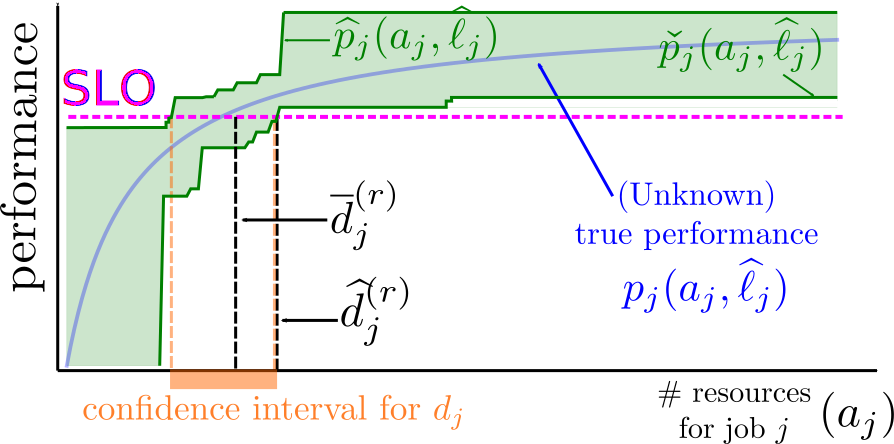
\includegraphics[width=4.1in]{cilantro/figs/algo_illus/mmflearn_opt.pdf}
\vspace{-0.1in}
\caption{ 
Illustration of Cilantro's uncertainty-aware demand-based policies.
We first obtain a UCB $\volhatj$ from the load forecaster, which ensures
that we have a conservative estimate on the job's load.
In the figure, the $x$ axis is the amount of resources $\allocj$ that could be allocated to job $j$.
We show the SLO (pink),
the slice of the unknown performance curve (blue) when the load is $\volhatj$,
and the confidence region obtained from past data (green).
The LCB $\payoffcheckj$ and UCB $\payoffhatj$
on $\payoffj(a, \volhatj)$ are given by the lower and
upper boundaries of the confidence region (solid green lines).
A confidence interval for the demand (orange) can be obtained by the region where
$\payoffhatj,\payoffcheckj$ intersect the SLO line.
To obtain a recommendation, we compute a UCB $demhatjr$ on the demand (where SLO intersects
%\vspace{-0.05in}
$\payoffcheckj$) and $\dembarjr$ via equation~\eqref{eqn:ofudemand}.
% \rbcomment{Should we label y axis. Aren't $\payoffhatj$ and $\payoffcheckj$ incorrectly labelled}
\label{fig:demandrecillus}
% \vspace{-0.05in}
}
\end{figure}
}

\newcommand{\insertFigUtilityIllus}{
\begin{figure*}
\centering
\includegraphics[height=1in]{cilantro/figs/utility_curves/utility_curve_all_toplegend.pdf} %height = 1.1 for top legend, 0.8 for side legend
\vspace{-0.25in}
\caption{ 
Three candidates for SLO-based utility functions.
The left-most figure shows a job's performance $\payoffj$ as a function of the resources (for fixed
load).
In (a), the utility scales linearly with performance until the SLO,
i.e  $\utilpj(\payoff) \propto \min(\payoff, \textrm{SLO})$, whereas in
(b) it scales quadratically $\utilpj(\payoff) \propto \min(\payoff, \textrm{SLO})^2$,
and in (c) it scales with the square-root $\utilpj(\payoff) \propto \min(\payoff, \textrm{SLO})^{\nicefrac{1}{2}}$.
Here,
(b) captures settings where even small SLO violations are critical while (c) captures settings
where small SLO violations are not very significant.
% (a) The utility scales linearly with performance until the SLO.
% (a) The utility scales linearly with performance until the SLO.
% An SLO-aware utility (blue curve, $y$-axis on right) derived from the raw
% performance metric (red curve, $y$-axis on left).
% While we have used this form of utilities for our evaluation in this work,
% \cilantros can handle most utilities which are non-decreasing in the raw performance metric.
\label{fig:utilityillus}
\vspace{0in}
}
\end{figure*}
}

% \newcommand{\insertFigUtilityIllus}{
% \begin{figure}
% \centering
% \includegraphics[width=2in]{cilantro/figs/payoffillus_v2}
% \vspace{-0.1in}
% \caption{ 
% An SLO-aware utility (blue curve, $y$-axis on right) derived from the raw
% performance metric (red curve, $y$-axis on left).
% While we have used this form of utilities for our evaluation in this work,
% \cilantros can handle most utilities which are non-decreasing in the raw performance metric.
% \label{fig:utilityillus}
% \vspace{-0.1in}
% }
% \end{figure}
% }

\newcommand{\insertFigStrategyCompare}{
\begin{figure*}
\centering
% \begin
\hspace{-1.02in}
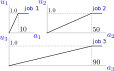
\includegraphics[width=1.45in]{cilantro/figs/strategy_compare}
\hspace{0.01in}
\begin{minipage}[t]{3.9in}
\footnotesize
\vspace{-1.05in}
\begin{tabular}{l||cc|cc|cc||c|c|c}
 & \multicolumn{6}{c||}{allocation (utility)}  & \multicolumn{3}{c}{metrics} \\
Policy & \multicolumn{2}{c|}{job 1} & \multicolumn{2}{c|}{job 2} & \multicolumn{2}{c||}{job 3}
& $\socwel$ & $\egalwel$ & $\njcfair$
\\ \midrule
Social welfare & 10 & (1.0) & 50 & (1.0) & 0 & (0.0) & 0.67 & 0.0 & 0.0 \\
Egalitarian welfare & 4 & (0.4) & 20 & (0.4) & 36 & (0.4)  & 0.4 & 0.4 & 0.4 \\
NJC fair & 10 & (1.0) & 25 & (0.5) & 25 & (0.28) & 0.59 & 0.28 & 1.0 \\
Resource fair & 20 & (1.0) & 20 & (0.4) & 20 & (0.22) & 0.54 & 0.22 & 1.0 \\
\end{tabular}
\end{minipage}
\vspace{-0.1in}
\caption{ 
\cameratext{Comparison of the three (oracular) fair allocation criteria described in \S\ref{sec:oracularpolicies}
in a synthetic example with $60$ CPUs.
\emph{Left:} Utility curves for three jobs. The $y$ axis is the utility
and the $x$-axis is the number of resources.
For simplicity, we have ignored the loads and assumed that utilities increase
linearly up to the demand.
The total demand is 150, whereas only 60 resources are available.
% hence, an allocation policy should decide how best to divide the resources.
\emph{Right:} The allocations and utilities for each job under
the three criteria.
% for the social welfare maximizing policy (Soc. welf.), egalitarian welfare
% maximizing policy (Egal. welf.), the NJC fairness policy (NJC fair.) and when 
% allocating the resources equally (Equal).
We have also shown the $\socwel$~\eqref{eqn:socwel}, $\egalwel$~\eqref{eqn:egalwel},
and $\njcfair$~\eqref{eqn:njcfair} metrics for each policy.
% Different policies might be appropriate for different use cases.
% \cilantro{} provides tools to allocate according to many such policies including the above
%  when the utilities are unknown a priori.
% The correct policy might 
% \kkcomment{Is this example useful? Does it need more explanation?}
}
\label{fig:strategycompare}
% \vspace{-0.1in}
}
\end{figure*}
}


\newcommand{\insertFigSP}{
\begin{figure}[t]
\centering
\includegraphics[width=0.63\linewidth]{cilantro/figs/sp_results_nofonts.pdf}
\\
\includegraphics[width=0.7\linewidth]{cilantro/figs/sp_legend_nofonts.pdf}
\insertFigCaptionSpace
\vspace{-0.3in}
\caption{ 
The utility of \incmtt{db16} under the three online learning policies,
when they report truthfully,
when they under-report, and
when they over-report.
The plot normalizes with respect to truthful reporting, but the bars are
annotated with the absolute value.
%\vspace{-0.2in}
\label{fig:spness}
\insertFigCaptionSpace
}
\end{figure}
}


\newcommand{\insertFigFallback}{
\begin{figure}[t]
\centering
\includegraphics[width=\linewidth]{cilantro/figs/fallback_results}
\\
\includegraphics[width=\linewidth]{cilantro/figs/fallback_legend}
\insertFigCaptionSpace
\vspace{-0.3in}
\caption{ 
Evaluation of Cilantro's fallback option, where users provide a demand value if they cannot
report performance metrics.
We evaluate \cilantronjcs when 
5 out of 20 users use this option.
Since the true demand cannot be known, we use either half or twice the true demand under the median
load from our profiled data.
% \vspace{-0.1in}
\label{fig:fallback}
\insertFigCaptionSpace
}
\end{figure}
}

\newcommand{\insertResUtilIllus}{
\begin{figure}
\centering
% Source: https://github.com/romilbhardwaj/mmflearn/tree/tpcds/mmflearn/exp/serving
% \includegraphics[width=\linewidth]{cilantro/figs/resource_qps_bin_combined_nsdi23.pdf}
\includegraphics[width=0.8\linewidth]{cilantro/figs/resource_qps_bin_combined_osdi23.pdf}
% \includegraphics[width=1.5in]{cilantro/figs/resource_qps_bin0.pdf}
% \hspace{0.1in}
% \includegraphics[width=1.5in]{cilantro/figs/resource_qps_bin1.pdf}
\vspace{-0.1in}
\caption{ 
Two users, \cameratext{U1 and U2}, serving TPC-DS benchmark queries with different resource-throughput mappings and 
performance goals (SLO).
% While the users' throughput may increase when she receives more resources, their utility
% is clipped at their SLOs.
A user's demand is the amount of CPUs needed for her SLO.
% A 50-50 fair allocation of resources causes user 2 to miss their SLO, while user 1 has already exceeded their SLO.
\label{fig:toyexample}
% \vspace{-0.25in}
}
\end{figure}
}


\newcommand{\insertFigMetrics}{
\begin{figure*}[!t]
\centering
% \includegraphics[width=3.5in]{cilantro/figs/util_drawing.png}
\includegraphics[width=2.9in]{cilantro/figs/util_vs_fairness_nofonts.pdf}
\hspace{0.4in}
\includegraphics[width=2.9in]{cilantro/figs/egal_vs_fairness_nofonts.pdf}
\\[0.05in]
\vspace{0.1in}
\includegraphics[width=6.5in]{cilantro/figs/welf_vs_fairness_legend_nofonts.pdf}
% \vspace{-0.1in}
\vspace{-0.15in}
\caption{ 
NJC fairness vs the social and egalitarian welfare
(see~\S\ref{sec:oracularpolicies}) for all policies.
We report the average value over the 6 hour period.
Higher is better for all metrics, so closer to the top right corner is  desirable.
The \oraclesw, \oracleew{} policies optimize for the social and egalitarian welfare when the
performance mappings are known and \oraclenjc{} achieves maximum fairness
 while improving
cluster usage. The corresponding \cilantros policies are designed to do the same without a priori
knowledge of the performance mappings.
% \rbcomment{Can we reduce the height of this figure and add grids (plt.grid()). Also increase x and y label font sizes?}
\label{fig:metrics}
}
% \vspace{-0.1in}
\end{figure*}
}

\newcommand{\convergencewidthleg}{5.2in}
\newcommand{\convergencewidth}{5in}
\newcommand{\insertFigTimeseriesUtilities}{
\begin{figure}
\centering
% \includegraphics[width=3.5in]{cilantro/figs/util_drawing.png}
\includegraphics[width=\convergencewidthleg]{cilantro/figs/timeseries_results/ts_legend_nofonts.pdf}
\\[-0.07in]
\includegraphics[width=\convergencewidth]{cilantro/figs/timeseries_results/util_welfare_long_nofonts.pdf}
\includegraphics[width=\convergencewidth]{cilantro/figs/timeseries_results/egal_welfare_long_nofonts.pdf}
\includegraphics[width=\convergencewidth]{cilantro/figs/timeseries_results/max_fairness_viol_long_nofonts.pdf}
\vspace{-0.1in}
\caption{ 
Convergence over time of social, egalitarian welfares and NJC fairness for the three Cilantro policies.
\label{fig:timeseriesutilities}
}
% \vspace{-0.2in}
\end{figure}
}

\newcommand{\profwidth}{1.5in}
\newcommand{\profhspace}{0.05in}
\newcommand{\insertFigProfiling}{
\begin{figure*}[!t]
\centering
% \includegraphics[width=3.5in]{cilantro/figs/util_drawing.png}
\includegraphics[width=\profwidth]{cilantro/figs/prof_craydb0_nofonts.pdf}
\hspace{\profhspace}
\includegraphics[width=\profwidth]{cilantro/figs/prof_craydb1_nofonts.pdf}
\hspace{\profhspace}
\includegraphics[width=\profwidth]{cilantro/figs/prof_craypredserv_nofonts.pdf}
\hspace{\profhspace}
\includegraphics[width=\profwidth]{cilantro/figs/prof_craymltrain_nofonts.pdf}
\vspace{-0.1in}
\caption{ 
Performance vs resource-allocation-per-unit-load 
obtained after profiling the database querying, predicition serving and ML training workloads. %described in \S\ref{sec:fixedclus} for \~9 hours.
% The resource to performance mappings obtained via the adaptive binning estimator
% (see Sec.~\ref{sec:method}) for the four workloads after approximately $6$ hours of
% profiling.
% after profiling each workload for approximately 4 hours.
The blue curve is the average performance value and the shaded region is the 2$\sigma$ confidence
interval.
% Shaded in blue is the $95\%$ (2-$\sigma$) confidence region for the average
% performance value and
% shaded in green is the $95\%$ region for the noisy performance value.
For the latency-based workloads (DB-0, DB-1, and prediction serving), we show the number of
resources per unit load (arrival QPS) on the $x$-axis and the fraction of queries completed
under 2s on the $y$-axis.
For the ML training workload, we show the number of resources on the $x$ axis the
amount of data processed per second on the $y$-axis.
To obtain accurate estimates, we sampled low resources allocations more
densely.
\label{fig:profiling}
% \vspace{-0.1in}
}
\end{figure*}
}


\newcommand{\insertFigUserUtilities}{
\begin{figure*}[!t]
\centering
% \includegraphics[width=3.5in]{cilantro/figs/util_drawing.png}
\includegraphics[width=6in]{cilantro/figs/util_plot_nofonts.pdf}
\\
\includegraphics[width=4in]{cilantro/figs/leg_util_plot_nofonts.pdf}
\vspace{-0.15in}
\caption{ 
The average utility achieved by the 20 jobs for the three online learning
methods in Cilantro and \equalshare.
Here, \incmtt{db0x}, \incmtt{mltx}, \incmtt{db1x}, and \incmtt{prsx}
refers to jobs using the DB-0, ML training, DB-1, and prediction
serving workloads from \S~\ref{sec:fixedclus}.
% \rbcomment{can we add horizontal grids (ax.grid(axis='y')?}
\label{fig:userutils}
% \vspace{-0.1in}
}
\end{figure*}
}

\newcommand{\insertFigMSResults}{
% \begin{figure*}
% \centering
% \begin{minipage}{2.0in}
% \vspace{-1.3in}
% \begin{tabular}{c|c}
% \toprule
% Policy & P99 Latency (ms) \\
% \midrule
% \equalshare &  $3014.232 \pm 24.04$ \\
% \msiles & $1459.45 \pm 45.99$ \\
% \msevoopts & $947.74 \pm 60.41$  \\
% \ucbopts &  $536.58 \pm 33.00$ \\
% \midrule
% \end{tabular}
% \end{minipage}
% \hspace{0.05in}
% \includegraphics[height=1.4in]{cilantro/figs/p99}
% \hspace{0.05in}
% \includegraphics[height=1.4in]{cilantro/figs/cum_p99}
% \vspace{-0.1in}
% \caption{ 
% Results for the microservices experiment comparing four methods on P99
% latency over 6 hours.
% \emph{Left:} The time-averaged P99 latency over the duration of the experiment.
% \emph{Mid:} The instantaneous P99 latency vs time. 
% \emph{Right:} The time-averaged P99 latency vs time.
% \rbcomment{Add subcaptions}
% \label{fig:microservices}
% }
% \vspace{-0.1in}
% \end{figure*}
% https://docs.google.com/drawings/d/1L6rxyGkY2bmtLTxUOTn_fVI9L4Sumbn6MQS9HXe_1lc/edit?usp=sharing
\begin{figure*}[t]
\begin{subfigure}[b]{0.35\textwidth}
\raisebox{3mm}{
     \includegraphics[width=\textwidth]{cilantro/figs/HotelServicesArch.pdf}
    %  \caption{}
     \label{fig:hotelresarch}
}
% % P99 Average table
% \footnotesize
% % \begin{table}[ht]
% % \begin{center}
% \raisebox{16mm}{
% \begin{tabular}{c|c}
% \toprule
% \textbf{Policy} & \textbf{P99 Latency (ms)} \\
% \midrule
% \equalshare &  $3014.232 \pm 24.04$ \\
% \msiles & $1459.45 \pm 45.99$ \\
% \msevoopts & $947.74 \pm 60.41$  \\
% \ucbopts &  $536.58 \pm 33.00$ \\
% \midrule
% \end{tabular}
% }
% \caption{}
\label{tab:msp99}
%\vspace{-8mm}
% \end{table}
\end{subfigure}
\hspace{2mm}
\begin{subfigure}[b]{0.3\textwidth}
\centering
\includegraphics[width=\textwidth]{cilantro/figs/p99_nofonts.pdf}
% \caption{}
\label{fig:msp99}
\end{subfigure}
\hspace{2mm}
\begin{subfigure}[b]{0.3\textwidth}
 \includegraphics[width=\textwidth]{cilantro/figs/cum_p99_nofonts.pdf}
%  \caption{}
 \label{fig:avgmsp99}
\end{subfigure}
\vspace{-8mm}
\caption{ 
\emph{Left:} Microservices architecture of the hotel reservation benchmark\cite{deathstarbench}. Blue boxes are business logic, red boxes are caching services, yellow boxes are databases and purple boxes are networking services.
\emph{Center:} Results for the microservices experiment comparing four methods on P99 latency over 6 hours, plotting the instantaneous P99 latency vs time.
\emph{Right:} The time-averaged P99 latency vs time.
\label{fig:microservices}
}
% \vspace{-0.1in}
\end{figure*}
}


% propfair::  p99= 3014.232 +/- 24.0379,    cum_p99= 2929.174 +/- 20.5772,    
% msile::  p99= 1459.452 +/- 45.9874,    cum_p99= 2129.006 +/- 26.1716,    
% msevoopt::  p99= 947.741 +/- 60.4008,    cum_p99= 1731.231 +/- 33.4763,    
% ucbopt::  p99= 536.577 +/- 33.0044,    cum_p99= 1294.783 +/- 34.3378,    




\newcommand{\insertFigUpdateFreq}{
\begin{figure}
\centering
% \includegraphics[width=3.5in]{cilantro/figs/util_drawing.png}
\includegraphics[width=0.8\linewidth]{cilantro/figs/update_freq}
\vspace{-0.1in}
\caption{ 
The frequency of performance updates (per hour) for
4 different users from the experiment in \S\ref{sec:fixedclus}.
% \label{fig:frequpdate}
}
% \vspace{-0.1in}
\end{figure}
}


\newcommand{\insertFigAutoScaling}{
\begin{figure}
\centering
% \includegraphics[width=3.5in]{cilantro/figs/util_drawing.png}
\includegraphics[width=0.8\linewidth]{cilantro/figs/autoscaling_db1}
\vspace{-0.1in}
\caption{ 
Cost (\# replicas) v time for the auto scaling experiment.
\label{fig:autoscaling}
}
% \vspace{-0.1in}
\end{figure}
}

\newcommand{\insertFigTwitterTrace}{
\begin{figure}[t]
    \centering
    \includegraphics[width=\linewidth]{cilantro/figs/twitter_trace_nofonts.pdf}
    \caption{Sampled query arrival rate from the twitter trace collected over the duration of a day.}
    \label{fig:twitter_trace}
\end{figure}
}

\newcommand{\insertFigHotelReservation}{
\begin{figure}
    \centering
    % https://docs.google.com/drawings/d/1L6rxyGkY2bmtLTxUOTn_fVI9L4Sumbn6MQS9HXe_1lc/edit?usp=sharing
    \includegraphics[width=0.85\linewidth]{cilantro/figs/HotelServicesArch.pdf}
    \vspace{-3mm}
    \caption{Microservices architecture of the hotel reservation benchmark\cite{deathstarbench}. Blue components indicate business logic implemented in Go. Red boxes indicate caching services, yellow boxes are databases and purple boxes are networking and tracing services.}
    \label{fig:hotelresarch}
    \vspace{-2mm}
\end{figure}
}


\newcommand{\insertFigMicrobenchmarks}{

\begin{figure*}[t]
    \begin{subfigure}[b]{0.22\textwidth}
    \tiny
    % \begin{table}[ht]
    % \begin{center}
    \raisebox{16mm}{
            % \begin{tabular}{c|c|c|c}
            % \toprule
            % %\getalloc{} for
            % \multirowcell{2}{Model \\ Update} & \multicolumn{3}{c}{\getalloc{} call time (s)} \\ \cline{2-4} 
            %  & \cilantrosw & \cilantroew & \cilantronjc\\
            % \midrule
            % %$0.0413 \pm 0.0048$ &  $2.8823 \pm 0.3155$ &  $2.1239 \pm 0.0212$ & $0.8132 \pm 0.162$ \\
            % $0.04 \pm 0.01$ &  $2.88 \pm 0.31$ &  $2.12 \pm 0.02$ & $0.81 \pm 0.16$ \\
            % \bottomrule
            % \end{tabular}
            \begin{tabular}{c|c}
            \toprule
            \textbf{Operation} & \textbf{Call time (s)} \\
            \midrule
            Model Update & $0.0413 \pm 0.0048$ \\
            \midrule
            \incmtt{get-alloc} call \\
            \cilantrosw  & $2.8823 \pm 0.3155$ \\
            \cilantroew  & $2.1239 \pm 0.0212$ \\
            \cilantronjc & $0.0081 \pm 0.0016$ \\
            \bottomrule
            \end{tabular}
    }
%     \caption{}
    \label{tab:mbtime}
    %\vspace{-8mm}
    % \end{table}
    \end{subfigure}
    \hspace{12mm}
    \begin{subfigure}[b]{0.45\textwidth}
    \centering
        \includegraphics[width=\linewidth]{cilantro/figs/fallback_legend_nofonts.pdf}
        \\
        \includegraphics[width=\linewidth]{cilantro/figs/fallback_results_nofonts.pdf}
%         \caption{}
    \label{fig:fallback}
    \end{subfigure}
%     \hspace{1mm}
%     \begin{subfigure}[b]{0.25\textwidth}
%          \raisebox{0.5mm}{
%             \includegraphics[width=\textwidth]{cilantro/figs/update_freq}
%          }
%          \caption{}
%      \label{fig:frequpdate}
%     \end{subfigure}
    \hspace{-3mm}
    \begin{subfigure}[b]{0.23\textwidth}
         \raisebox{0mm}{
            \includegraphics[width=\textwidth]{cilantro/figs/error_mb_line_nofonts.pdf}
         }
%          \caption*{}
     \label{fig:frequpdate}
    \end{subfigure}
    \vspace{-8mm}
    \caption{ 
    Cilantro microbenchmarks.
\emph{Left:} Mean time taken (in seconds) by \cilantro{} to update the performance model and for
computing a new allocation for each of the three fixed cluster sharing policies. 
\emph{Center:} Evaluation of Cilantro's fallback option, where users provide a demand value if they cannot report performance metrics.
We evaluate \cilantronjcs when 5 out of 20 users use this option. Since the true demand cannot be known, we use either half or twice the true demand under the median load from our profiled data.
% (right) The frequency of performance updates (per hour) for 4 different users from the experiment in \S\ref{sec:fixedclus}.
\emph{Right:} The three performance metrics for \cilantronjcs when we artificially introduce error to the
confidence intervals of the performance and load.
    % \vspace{-0.1in}
    \label{fig:microbenchmarks}
    }
\end{figure*}
}

% https://docs.google.com/drawings/d/1C6wa4tSfnMBdx-0mlUtxPS3jWeufVjNxWFNhGJlR09c/edit?usp=sharing
\newcommand{\insertFigCilantroOverview}{
\begin{figure}
    \centering
    \includegraphics[width=4.5in]{cilantro/figs/cilantro_simple_arch.pdf}
    \vspace{-2mm}
    \caption{
    Cilantro overview. Cilantro uses continuous feedback to dynamically learn each job's
    resource-to-performance mappings.
    An uncertainty-aware resource allocation policy,
    instantiated for the user's objective,
    uses these mappings to determine allocations.
%     The decoupling of l
}
    \label{fig:cilantrooverview}
    % \vspace{-0.15in}
\end{figure}
}

% https://docs.google.com/drawings/d/1C6wa4tSfnMBdx-0mlUtxPS3jWeufVjNxWFNhGJlR09c/edit?usp=sharing
\newcommand{\insertFigMicrobenchmarkSchedLatency}{
\begin{figure}
    \centering
    \includegraphics[width=3.2in]{cilantro/figs/sched_latency.pdf}
    \vspace{-1mm}
    \caption{Scheduling latency in Cilantro with varying number of jobs. Even with 10000 jobs, the total time taken to allocate resources for all jobs remains less than 110ms. \rbcomment{Switch to box plot instead of violin? Add text in paper. Also seems to be inconsistent with 12a. Remove, move data to text.}}
    \label{fig:schedlatency}
    % \vspace{-2mm}
\end{figure}
}
